\documentclass{article}

\usepackage{fullpage}
\usepackage{graphicx}
\usepackage{amsmath}
\usepackage{grffile}

\begin{document}

\title{Regularity of Equilibrium Cell Number Density $\rho(n)$ at $n=0$}
\author{}
\date{}

\maketitle

\noindent In this report, we investigate the regularity of the equilibrium cell number density $\rho(n)$ at $n=0$ for the continuous-time spatially-discretized diffusion-only system (i.e., set of SODEs).
We recall that, in the previous report, it is expected that under the condtion
\begin{equation}
\label{cond}
\tilde{n}(n_1,n_2) = 0\quad\mbox{for $n_1<0$ or $n_2<0$},
\end{equation}
$\rho(n)$ does not allow negative density and the regularity of $\tilde{n}(n_1,n_2)$ at $n_1=0$ or $n_2=0$ may affect that of $\rho(n)$ at $n=0$.
Condition~\eqref{cond} can be implemented by multiplying $H(n_1)H(n_2)$ or $H(\mathrm{min}(n1,n2))$, where $H(n)$ is the Heaviside step function.
However, especially for the arithmetic average $\frac{1}{2}(n_1+n_2)$, this causes discontinuity in $\tilde{n}(n_1,n_2)$ and, as a remedy, $H(n)$ is replaced by a \textit{smoothed} Heaviside step function.
In the current code, the following form of $\tilde{n}(n_1,n_2)$ is implemented:
\begin{equation}
\label{tildencode}
\tilde{n}(n_1,n_2) = \frac{1}{2}(n_1+n_2)H_\infty(\mathrm{min}(n_1,n_2)),
\end{equation}
where $H_\infty(n)$ is constructed by using the hyperbolic tangent function.
In order to investigate the regularity change on $\rho(n)$ depending on $\tilde{n}(n_1,n_2)$, we employ $C_k$-smoothed Heaviside step functions $H_k(n)$ ($k=0,1,2$) as well as the (discontinuous) Heaviside step $H(n)$ and use 
\begin{equation}
\label{tildenCk}
\tilde{n}(n_1,n_2) = \frac{1}{2}(n_1+n_2)H_*(n_1) H_*(n_2),
\end{equation}
where $H_*$ is $H$, $H_0$, $H_1$, or $H_2$.
Smoothed Heaviside functions $H_k$ are constructed as follows: 
\begin{equation}
H_k(n)=\begin{cases} 
0 & n<0,\\
p_{2k-1}\left(n\Delta V\right) & 0\le n\Delta V\le 1,\\
1 & n\Delta V>1.
\end{cases}
\end{equation}
Here, $p_{2k-1}(x)$ is a polynomial of order $2k-1$ and its $2k$ coefficients are determined from the $C_k$ smoothness condition of $H_k$.
Note that $\tilde{n}(n_1,n_2)$ given in Eq.~\eqref{tildenCk} preserves the regularity of $H_k$, whereas that in Eq.~\eqref{tildencode} does not because of the minimun function.

\section{Results}

For $\Delta V=5$, $\rho(n)$ is computed for $\tilde{n}(n_1,n_2)$ given in Eq.~\eqref{tildenCk} with $H$, $H_0$, $H_1$ and $H_2$ as well as $\tilde{n}(n_1,n_2)$ in Eq.~\eqref{tildencode}.
The results computed with a small time step $\Delta t=0.001$ are shown in Fig.~\ref{fig_dt0.001}.
As expected, the results obtained from $H$ and $H_0$ show that the regularity is not good in these cases. 
For $H$, $\rho(n)$ has a sharp peak in the small negative density region, which will be shown below to be a delta function in the limit $\Delta t\rightarrow 0$.
For $H_0$, although $\rho(n)$ is continuous at $n=0$, it does not seem differentiable at $n=0$.
On the other hand, for $H_1$ and $H_2$, $\rho(n)$ seems differentiable at $n=0$.
Hence, although we could not distinguish the two cases with $H_1$ and $H_2$, all observations are consistent with our conjecture that the regularity of $\rho(n)$ depends on that of $\tilde{n}(n_1,n_2)$.
However, note that it is not so straightforward to check the regularity of a function from its numerical values.
Moreover, in our case, we attemp to check our conjecture for the limit $\Delta t\rightarrow 0$ by numerical results with small $\Delta t$.
For the comparison of numerical results with different time step values ($\Delta t=0.001$ and 0.01), see Fig.~\ref{fig_comp_dt}.
For the (discontinuous) Heaviside function $H$, several values of $\Delta t =0.001$, 0.002, 0.005, 0.01 were used and the results are shown in Fig.~\ref{fig_avg4}.

\begin{figure}
\centering
\includegraphics[angle=270,width=0.75\linewidth]{fig5/DT0.001.eps}
\caption{\label{fig_dt0.001}The equilibrium cell number distribution $\rho(n)$ near $n=0$. A small time step $\Delta t=0.001$ is used.}
\end{figure}

\begin{figure}
\centering
\includegraphics[angle=270,width=\linewidth]{fig5/comp_dt.eps}
\caption{\label{fig_comp_dt}The equilibrium cell number distribution $\rho(n)$ near $n=0$. For each definition of $\tilde{n}(n_1,n_2)$, the profiles of $\rho(n)$ obtained from different values of $\Delta t$ are compared. The results for Heaviside step function $H$ are shown in Fig.~\ref{fig_avg4}.}
\end{figure}

\section{Delta function in $\rho(n)$}

\begin{figure}
\centering
\includegraphics[angle=270,width=\linewidth]{fig5/AVG4.eps}
\caption{\label{fig_avg4}The equilibrium cell number distribution $\rho(n)$ near $n=0$ for $\tilde{n}(n_1,n_2)$ with the Heaviside step function $H$. In the left panel, the profiles of $\rho(n)$ obtained from different values of $\Delta t$ are compared. In the right panel, a scaling behavior given in Eq.~\eqref{avg4_scaling} is tested for the sharp peak in the small negative denisty region.}
\end{figure}

In this section, we discuss the sharp peak of $\rho(n)$ which is present at the small number density region.
As shown in the left panel of Fig.~\ref{fig_avg4}, the height of the peak increases as $\Delta t$ decreases, whereas the support of the peak shrinks.
In addition, the total probability of negative density dose not change for different values of $\Delta t$.
This observation leads to test the following scaling behavior:
\begin{equation}
\label{avg4_scaling}
\rho(n)\approx \frac{1}{\sqrt{\Delta t}}f\left(\frac{n}{\sqrt{\Delta t}}\right)\quad\mbox{for $n<0$}.
\end{equation}
As shown in the right panel of Fig.~\ref{fig_avg4}, the agreement is remarkably good.
Eq.~\eqref{avg4_scaling} suggests that, if $H$ is used in Eq.~\eqref{tildenCk}, $\rho(n)$ has the following form in the limit $\Delta t\rightarrow 0$:
\begin{equation}
\lim_{\Delta t\rightarrow 0}\rho(n)=\rho_0(n)+A\delta(n),
\end{equation}
where $\rho_0(n)$ has nonzero values only for $n\ge0$.
For a possible explanation on the scaling behavior given in Eq.~\eqref{avg4_scaling}, see below the Appendix.

\section{Conclusion}

We confirm that our numerical results are consistent with the following conjecture:
\begin{itemize}
\item While Condition~\eqref{cond} is a crucial condition for non-negative density, the regularity condition of $\tilde{n}(n_1,n_2)$ is for the regularity of $\rho(n)$ at $n=0$.
\end{itemize}
In other words, as seen in the case of $H$, the equilibrium cell number density attains non-negative density.
However, due to the lack of regularity, $\rho(n)$ has a delta function at $n=0$. 

\section*{Appendix: Explanation of the form of $\rho(n)$ for $n<0$ in Eq.~\eqref{avg4_scaling}}

For sufficiently small $\Delta t>0$, the form of $\rho(n)$ for $n<0$ can be explained by the balance of the following probabilities in equilibrium:
\begin{align}
&P_1 = \mathrm{Prob}(n_1(0)>0\mbox{ and }n_1(\Delta t)<0),\\
&P_2 = \mathrm{Prob}(n_1(0)<0\mbox{ and }n_1(\Delta t)>0).
\end{align}
We express $P_1$ and $P_2$ in terms of $\rho^+=\lim_{n\downarrow 0}\rho(n)$ and $\rho^-=\lim_{n\uparrow 0}\rho(n)$.

Relevent events for $P_1$ occur when small $n_1$ becomes negative because of stochastic flux. 
Since the magnitude of stochastic flux is of order $\sqrt{\Delta t}$ whereas that of mean diffusion is of order $\Delta t$, it suffices to consider only the stochastic flux $F$:
\begin{equation}
F=\frac{1}{\Delta x}\sqrt{\frac{2\chi\Delta t}{\Delta V}}\left(\sqrt{\frac{n_1+n_2}{2}}W_{1,2}-\sqrt{\frac{n_1+n_{N_\mathrm{c}}}{2}}W_{1,N_\mathrm{c}}\right).
\end{equation}
Since $n_1$ is small and $\langle n_2|n_1\rangle = \langle n_{N_\mathrm{c}}|n_1\rangle \approx \bar{n}$, we have
\begin{equation}
v\equiv\mathrm{Var}[F] \approx \frac{2\chi\bar{n}\Delta t}{\Delta x^2\Delta V}.
\end{equation}
By noting that $F$ is normally distributed, the probability $p(n_1)$ that $n_1$ becomes negative after time $\Delta t$ (that is, $n_1+F<0$) is given as
\begin{equation}
p(n_1)=\Phi\left(-\frac{n_1}{\sqrt{v}}\right),
\end{equation}
where $\phi(x)$ is the cumulative distribution function of the standard normal distribution.
Since $v=\mathrm{Var}[F]$ is of order $\Delta t$, the range of $n_1$ that contributes to $P_1$ is $0<n_1<\mathrm{O}(\sqrt{\Delta t})$.
Hence, we have
\begin{equation}
\label{P1}
P_1 = \int_0^\infty dn_1\; \rho(n_1)p(n_1)\approx \int_0^{\mathrm{O}(\sqrt{\Delta t})}dn\; \rho^+ p(n_1) = \rho^+ \sqrt{v}\alpha,
\end{equation}
where
\begin{equation}
\alpha = \int_0^\infty dy \int_{-\infty}^{-y}dx\frac{1}{\sqrt{2\pi}}e^{-x^2/2}=\frac{1}{\sqrt{2\pi}}.
\end{equation}

For $P_2$, the mean diffusion acts the main role.
Since the stochastic flux is turned off for $n_1<0$, $n_1$ is actually affected only by the diffusion.
Under the condition that $n_1$ is (negatively) small and $\langle n_2|n_1\rangle = \langle n_{N_\mathrm{c}}|n_1\rangle \approx \bar{n}$, we have
\begin{equation}
\dot{n}_1 = \chi\frac{n_2+n_{N_\mathrm{c}}-2n_1}{\Delta x^2}\approx\frac{2\chi\bar{n}}{\Delta x^2}.
\end{equation}
Hence, if $n_1$ satisfies the following condition, $n_1$ becomes positive after time $\Delta t$: 
\begin{equation}
n_1+\frac{2\chi\bar{n}}{\Delta x^2}\Delta t>0.
\end{equation}
Then, $P_2$ is approximated as
\begin{equation}
\label{P2}
P_2 = \int_{-\frac{2\chi\bar{n}}{\Delta x^2}\Delta t}^0 \rho(n_1) dn_1 \approx \frac{2\chi\bar{n}\Delta t}{\Delta x^2}\rho^-.
\end{equation}
Note that we assume that $\rho(n_1)\approx \rho^-$ on the interval $[-\mathrm{O}(\Delta t),0)$.
This is because the support of $\rho(n_1)$ for $n_1<0$ is $-\mathrm{O}(\sqrt{\Delta t})<n_1<0$.

By equating Eqs.~\eqref{P1} and \eqref{P2}, we obtain
\begin{equation}
\frac{\rho^-}{\rho^+}=\frac{1}{\sqrt{4\pi\chi\bar{n}}}\frac{\Delta x}{\sqrt{\Delta V}\Delta t}.
\end{equation}
This shows that the magnitude of $\rho(n_1)$ for $n_1<0$ grows like $\Delta t^{-1/2}$.
Note that we have explained why the support of $\rho(n_1)$ for $n_1<0$ is $-\mathrm{O}(\sqrt{\Delta}t)<n_1<0$; it is mainly because $v=\mathrm{Var}[F]$ is of order $\Delta t$.
Hence, we have explained the form of $\rho(n_1)$ for $n_1<0$ given in Eq.~\eqref{avg4_scaling}.

\end{document}
